%%%%%%%%%%%%%%%%%%%%%%%%%%%%%%%%%%%%%%%%%%%%%%%%%%%%%%%%%%%%%%%%%%%%
%% %%	Posterdown PDF class for LaTeX files	 08-JAN-2019
%% %%	For any information please send an e-mail to:
%% %%		brentthonre18@gmail.com (Brent Thorne)
%% %%
%% %%	Initial class provided by:
%% %%		Brent Thorne
%%%%%%%%%%%%%%%%%%%%%%%%%%%%%%%%%%%%%%%%%%%%%%%%%%%%%%%%%%%%%%%%%%%%

\documentclass[article,30pt,extrafontsizes]{memoir}

%utf-8 seems to be important
\RequirePackage[utf8]{inputenc}
\RequirePackage[T1]{fontenc}
\RequirePackage{lmodern}
\RequirePackage{multicol}
\RequirePackage{graphicx}
\RequirePackage{blindtext}
\RequirePackage[svgnames,table]{xcolor}
\RequirePackage{tikz}
\RequirePackage[framemethod=tikz]{mdframed}
\RequirePackage{color}
\RequirePackage{geometry}
\RequirePackage{adjmulticol}
\RequirePackage{epstopdf}
\RequirePackage{stfloats}
\RequirePackage[export]{adjustbox}

%For kable extra package :)
\RequirePackage{booktabs}
\RequirePackage{longtable}
\RequirePackage{array}
\RequirePackage{multirow}
\RequirePackage{wrapfig}
\RequirePackage{float}
\RequirePackage{colortbl}
\RequirePackage{pdflscape}
\RequirePackage{pagecolor}
\RequirePackage{tabu}
\RequirePackage{threeparttable}
\RequirePackage{threeparttablex}
\RequirePackage[normalem]{ulem}
\RequirePackage{makecell}
\RequirePackage{wrapfig}

%%%%%%%%% COLOURS %%%%%%%%

%Fill/ Line Colours
\definecolor{titlebgcol}{HTML}{690F8C}
\definecolor{columnlinecol}{HTML}{000000}
\definecolor{posterbgcol}{HTML}{ffffff}
\definecolor{headerbgcol}{HTML}{008080}

% Text Colours
\definecolor{titletextcol}{HTML}{ffffff}
\definecolor{authortextcol}{HTML}{DCDCDC}
\definecolor{affiliationtextcol}{HTML}{A1A1A1}
\definecolor{headertextcol}{HTML}{CC0000}
\definecolor{bodytextcol}{HTML}{000000}
\definecolor{footnotetextcol}{HTML}{FFFFFF}
\definecolor{citecol}{HTML}{CC0000}
\definecolor{urlcol}{HTML}{008080}
\definecolor{linkcol}{HTML}{008080}

\RequirePackage{hyperref}
\hypersetup{
    colorlinks=true,
    linkcolor=linkcol,
    citecolor=citecol,
    filecolor=magenta,
    urlcolor=urlcol,
}

%For figure and table placement
\RequirePackage{float}
\floatplacement{figure}{H}
\floatplacement{table}{H}

%spacing between figure/ table and caption
\setlength{\abovecaptionskip}{0.4in}
\setlength{\belowcaptionskip}{0.2in}
\captionnamefont{\footnotesize\sffamily\bfseries}
\captiontitlefont{\footnotesize\sffamily}

%define column options
\setlength{\columnseprule}{1pt}
\def\columnseprulecolor{\color{columnlinecol}}

\setsubsubsecheadstyle{\small\color{headertextcol}\textbf}% Set \section style
\setsecheadstyle{\small\color{headertextcol}}
\setsecnumformat{}
\def\sectionmark#1{\markboth{#1}{#1}}

%-----------------------------------------------------

\thispagestyle{empty}
\definecolor{light-gray}{gray}{0.9}

%biblatex options
\RequirePackage[sorting=none,backend=biber]{biblatex}
\renewcommand*{\bibfont}{\tiny}
\bibliography{MyLibrary}
\defbibheading{bibliography}[\bibname]{%
\setlength\bibitemsep{0.75\itemsep}
\section*{#1}%
\markboth{#1}{#1}}
\AtBeginDocument{%
  \renewcommand{\bibname}{References}
}

%bring in the users information
\author{Shea P. Connell\textsuperscript{1}, Marcel Hanna\textsuperscript{1},
Frank McCarthy\textsuperscript{2}, Rachel Hurst\textsuperscript{1},
Helen Curley\textsuperscript{1}, Martyn Webb\textsuperscript{1}, Helen
Walker\textsuperscript{3}, Rob Mills\textsuperscript{3}, Richard Y.
Ball\textsuperscript{3}, Martin G. Sanda\textsuperscript{4}, Kathryn L.
Pellegrini\textsuperscript{4}, Dattatraya Patil\textsuperscript{4},
Antoinette S. Perry\textsuperscript{5}, Jack
Schalken\textsuperscript{6}, Hardev Pandha\textsuperscript{7}, Hayley
Whitaker\textsuperscript{8}, Nening Dennis\textsuperscript{2}, Christine
Stuttle\textsuperscript{2}, Ian G. Mills\^{}9, 10, 11\^{}, Ingrid
Guldvik\textsuperscript{10}, The Movember Urine Biomarker Consortium,
Chris Parker\^{}12, 13\^{}, Jeremy Clark\textsuperscript{1}, Daniel S.
Brewer\^{}1, 13\^{}, Colin S. Cooper\textsuperscript{1}}
\title{\fontfamily{phv}\selectfont Predicting outcome in prostate cancer
patients using a multi-signature risk classifier, derived from urinary
extracellular vesicles}
\counterwithout{section}{chapter}
\makechapterstyle{mydefault}{
\addtocounter{secnumdepth}{2}
\setsecheadstyle{\centering\Large\color{headertextcol}\textbf}
\setsubsecheadstyle{\itshape}
\setsubsubsecheadstyle{\itshape}
}

\chapterstyle{mydefault}

%define column spacing
\setlength\columnsep{1in}

\setlength\parindent{1em}
\setlength\parskip{1em}
\setlength\hangparas{0}

%spacing after section head title
\setaftersecskip{0.3in}
\setbeforesecskip{1in}
\setlength\textfloatsep{0.3in}
\setlength\floatsep{0.3in}
\setlength\intextsep{0.3in}

\setstocksize{140cm}{90cm}
\settrimmedsize{\stockheight}{\stockwidth}{*}
\settypeblocksize{140cm}{90cm}{*}
\setlrmargins{*}{*}{1}
\setulmarginsandblock{2.5cm}{*}{*}
\setmarginnotes{0em}{0cm}{0cm}
\setlength{\footskip}{0cm}
\setlength{\footnotesep}{0cm}
\setlength{\headheight}{0pt}
\setlength{\headsep}{0pt}
\setlength{\trimtop}{0pt}
\setlength{\trimedge}{0pt}
\setlength{\uppermargin}{0pt}
\checkandfixthelayout

\mdfdefinestyle{brentsmdfstyle}{%
  backgroundcolor=titlebgcol,
  linecolor=columnlinecol,
  topline=false,
  leftline=false,
  rightline=false,
  linewidth=2mm}

%Footnote to white
\RequirePackage{footmisc}
\def\footnotelayout{\centering\color{footnotetextcol}}

% see https://stackoverflow.com/a/47122900

% choose font family
\RequirePackage{palatino}

\newpagecolor{posterbgcol}

%begin the document
\begin{document}
\begin{flushleft}
\begin{mdframed}[style=brentsmdfstyle]

%sets footnote to be white hopefully
\renewcommand\footnoterule{}
\renewcommand{\thempfootnote}{\footnotesize\color{footnotetextcol}{\arabic{mpfootnote}}}

% group which adds title author and other infor
% Used instead of \maketitle for better spacing options
\begingroup
  \centering
  \color{titletextcol}
\vspace{0.5in}
  \Huge{\fontfamily{phv}\selectfont Predicting outcome in prostate cancer
patients using a multi-signature risk classifier, derived from urinary
extracellular vesicles}  \\[0.3in]
  \color{authortextcol} \normalsize{Shea P. Connell\textsuperscript{1}, Marcel Hanna\textsuperscript{1},
Frank McCarthy\textsuperscript{2}, Rachel Hurst\textsuperscript{1},
Helen Curley\textsuperscript{1}, Martyn Webb\textsuperscript{1}, Helen
Walker\textsuperscript{3}, Rob Mills\textsuperscript{3}, Richard Y.
Ball\textsuperscript{3}, Martin G. Sanda\textsuperscript{4}, Kathryn L.
Pellegrini\textsuperscript{4}, Dattatraya Patil\textsuperscript{4},
Antoinette S. Perry\textsuperscript{5}, Jack
Schalken\textsuperscript{6}, Hardev Pandha\textsuperscript{7}, Hayley
Whitaker\textsuperscript{8}, Nening Dennis\textsuperscript{2}, Christine
Stuttle\textsuperscript{2}, Ian G. Mills\^{}9, 10, 11\^{}, Ingrid
Guldvik\textsuperscript{10}, The Movember Urine Biomarker Consortium,
Chris Parker\^{}12, 13\^{}, Jeremy Clark\textsuperscript{1}, Daniel S.
Brewer\^{}1, 13\^{}, Colin S. Cooper\textsuperscript{1}} \\[0.2in]
  \color{affiliationtextcol} \footnotesize{\textsuperscript{1} Norwich Medical School, University of East Anglia,
UK; \textsuperscript{2} The Institute of Cancer Research, UK;
\textsuperscript{3} Norfolk and Norwich University Hospitals NHS
Foundation Trust, UK; \textsuperscript{4} Department of Urology, Winship
Cancer Institute, Emory University School of Medicine, USA;
\textsuperscript{5} Cancer Biology and Therapeutics Laboratory, School
of Biology and Environmental Science, Conway Institute, University
College Dublin, Ireland; \textsuperscript{6} Nijmegen Medical Centre,
Radboud University Medical Centre, The Netherlands; \textsuperscript{7}
Faculty of Health and Medical Sciences, The University of Surrey, UK;
\textsuperscript{8} Molecular Diagnostics and Therapeutics Group,
University College London, UK; \textsuperscript{9} School of Medicine,
Dentistry and Biomedical Sciences, Institute for Health Sciences, Centre
for Cancer Research and Cell Biology, Queen's University Belfast, UK;
\textsuperscript{10} Centre for Molecular Medicine, University of Oslo,
Norway; \textsuperscript{11} Nuffield Department of Surgical Sciences,
University of Oxford, UK; \textsuperscript{12} The Royal Marsden
Hospital, Sutton, UK; \textsuperscript{13} The Earlham Institute,
Norwich Research Park, UK}
  \vspace{0.2in}

% end title section -------------------
  \endgroup
\end{mdframed}

%include the 4-Risk plots:
\graphicspath{ {Figures/} }
\begin{figure}
  \centering
  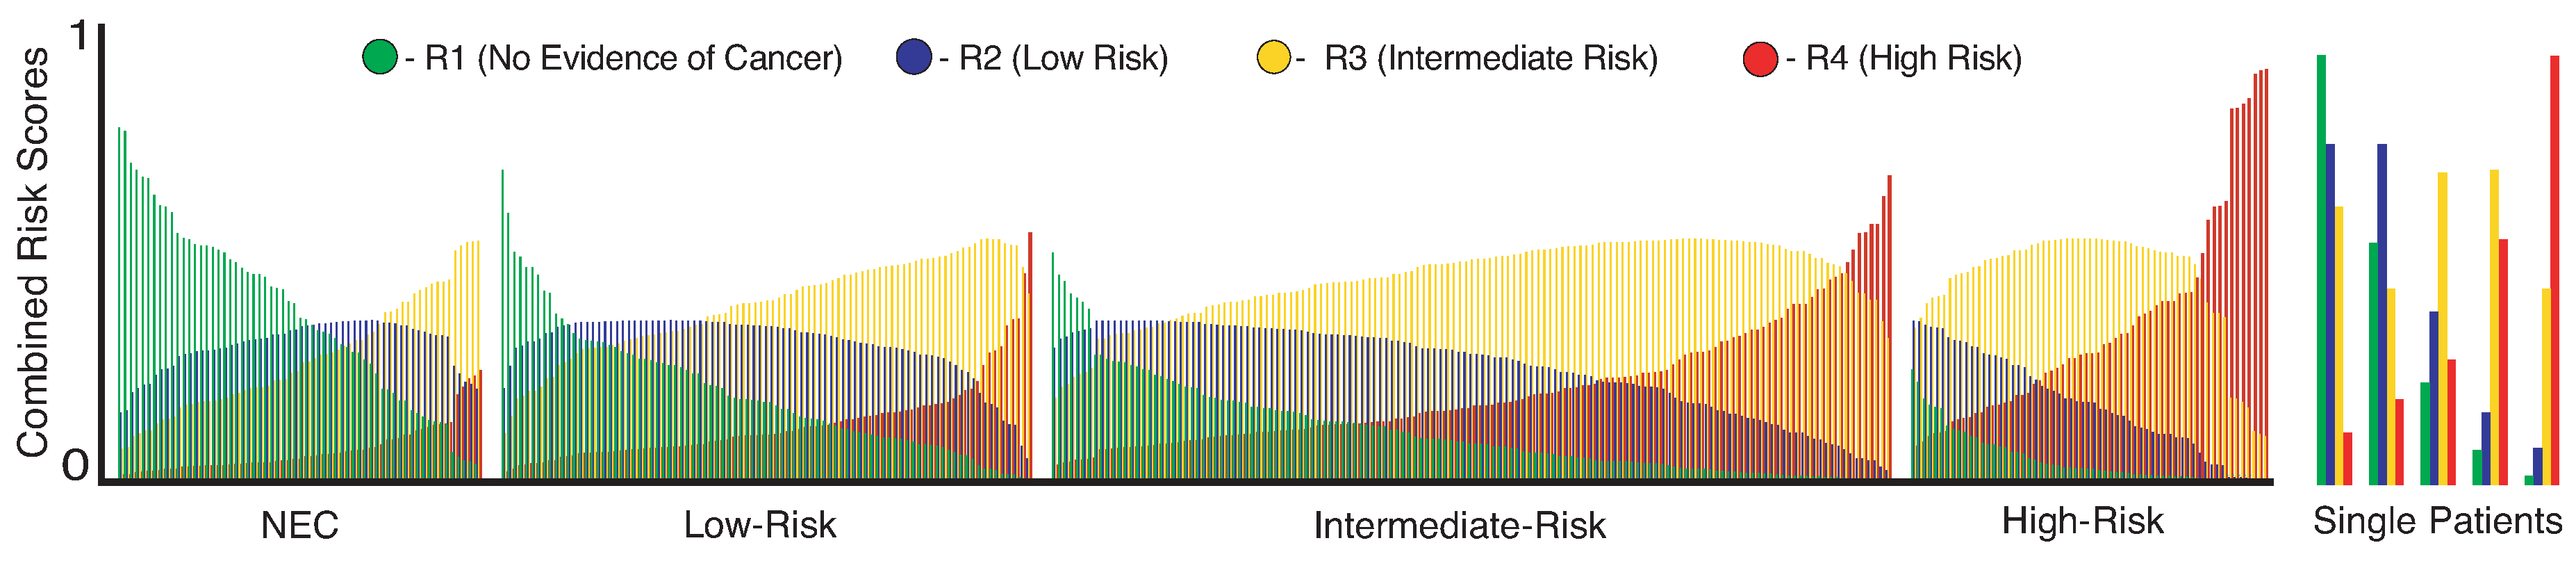
\includegraphics[width=80cm]{RiskProfiles}
\end{figure}
% Brgin body of poster
\begin{adjmulticols*}{2}{10mm}{10mm}
\normalsize{
\color{bodytextcol}
\definecolor{bordercolour}{HTML}{DCDCDC}
\definecolor{titleColour}{HTML}{252525}
\mdfsetup{frametitlealignment=\center,
          frametitlefont=\fontfamily{ppl}\selectfont,
          frametitlefont=\huge,
          frametitlebackgroundcolor=bordercolour,
          frametitlefontcolor = titleColour,
          linecolor=black,
          linewidth=5pt}
\definecolor{myframecolour}{HTML}{690F8C}
\begin{mdframed}[backgroundcolor = myframecolour,
                  font = \fontfamily{ppl}\selectfont,
                  fontcolor = white, 
                  roundcorner = 20pt, 
                  innerleftmargin = 30pt,
                  innerrightmargin = 30pt,
                  frametitle={\textbf{Quick Read:}}]
\large
\textbf{Question:} Can a non-invasive single-sample urine test reveal \textbf{both diagnostic and prognostic information} about 537 prostate cancer patients, utilising extracellular vesicle-derived RNA expression patterns? \\\\
\textbf{Findings:} A robust, four-risk-signature model identified two groups with differing rates of treatment intervention in active surveillance use (\textbf{High Risk HR = 3.7, Low Risk HR = -7.0}) and predicted initial biopsy outcome (\textbf{AUC = 0.81})\\\\
\textbf{Impact:} Clinical implementation of this model has the potential to avoid the unnecessary initial biopsy of men and the repeated, invasive follow-up of men on active surveillance with indolent prostate cancer could be drastically reduced, or provide a means for exiting surveillance altogether.\\
\end{mdframed}
\vspace{-40mm}

\hypertarget{introduction}{%
\section{Introduction}\label{introduction}}

Prostate cancer is estimated to be diagnosed in 12\% of men, the most
commonly diagnosed cancer in men in the
UK\autocite{CancerResearchUK2015}. However, 5-year survival of men with
prostate cancer is very high, and treatment of indolent, clinically
``irrelevant'' disease has significant side-effects, including
incontinence and impotence.

Men diagnosed with lower risk cancer are often placed on active
surveillance (AS) programmes, which have proven successful in improving
survival rates. Regardless, there is still no formal method for patients
on AS to exit these programmes.

Urine represents a suitable medium for non-invasively sampling the
prostate\autocites{McKiernan2016b}{Tomlins2016a}{Donovan2015}. In this
vain, we have developed a risk prediction model based on NanoString
quantified RNA expression in urinary extracellular vesicles, with the
aim to discriminate accurately between men with, and without, clinically
significant cancers. \vspace{-30mm}

\hypertarget{the-movember-cohort}{%
\section{The Movember Cohort:}\label{the-movember-cohort}}

\textbf{Patients:} 537 men with and without histologically proven cancer
with a PSA \textless{} 100 ng/mL, collected from urology clinics in the
UK, Ireland and USA between 2009 and 2015.

\textbf{Samples:} NanoString extracellular vesicular RNA expression
profiles of 167 gene-probes, derived from first-catch post-digital
rectal examination urine.

\textbf{AS Eligibility:} Age 50--80, clinical stage T1/T2, PSA
\textless{} 15 ng/mL, Gs \textless{}7 (Gs \textless{} 4+3 if age
\textgreater{}65), and \textless{}50\% percent positive biopsy cores.

\textbf{Progression:} PSA velocity \textgreater{}1 ng/mL per year or
adverse histology on repeat biopsy, defined as primary G \textgreater{}3
or \textgreater{}50\% biopsy cores positive for cancer

\vspace{-25mm}

\hypertarget{methods}{%
\section{Methods:}\label{methods}}

A continuation-ratio LASSO model was trained on 67\% of the data, using
D'Amico risk status as an ordinal variable, producing four risk
signatures for predicting the probability of normal tissue (R1), D'Amico
Low-risk (R2), Intermediate-risk (R3), and High-risk (R4) PCa in a given
sample.

This model was applied to the test dataset and to an AS sub-cohort (n =
87) for diagnostic and prognostic evaluation, respectively. ROC-AUC
analysis was used to test predicting biopsy outcome, and survival
analyses used to prognosticate the progression of patient in the AS
cohort. \vspace{-35mm}

\hypertarget{results}{%
\section{Results}\label{results}}

R4 was able to determine a clinically significant biopsy outcome of
D'Amico Intermediate- or High-Risk from a single urine sample, with an
\textbf{AUC = 0.813 (95\% CI: 0.779 - 0.847, Figure 1)}.

A robust R1 threshold dichotomised AS patients in to groups at low and
high risk of progression. The two groups had a large difference in time
to progression: 60\% progression within 5 years of urine sample
collection in the poor prognosis group compared to 10\% in the good
prognosis group (\(p\) \textless{} 0.001, log-rank test, Figure 2).

\begin{figure}

{\centering \includegraphics[width=1\linewidth,trim={0 5mm 0 10mm},clip]{Poster_files/figure-latex/unnamed-chunk-2-1} 

}

\caption{ROC-AUC plot of the ability of R4 to predict the presence of D'Amico Intermediate or High risk cancer on initial biopsy.}\label{fig:unnamed-chunk-2}
\end{figure}
\vspace{-10mm}

Cox proportional hazards models showed significant differences in
clinical outcome based on R1 or R4 of patients. The hazard ratio
associated with R4 was \textbf{3.71 (95\% CI: 1.53 to 5.89)}, with the
\textbf{HR of R1 =-7.03 (95\% CI: -12.29 to -1.77)}.

\begin{figure}

{\centering \includegraphics[width=1\linewidth,trim={0 2.5mm 0 2.5mm},clip]{Poster_files/figure-latex/unnamed-chunk-3-1} 

}

\caption{Kaplan-Meier plot of time to disease progression in months from initial urine collection. Colours indicate the dichotomised model thresholds, Green – High R1, Red – Low R1. Numbers above the x-axis indicate the number of patients in each group at risk at the given time intervals.}\label{fig:unnamed-chunk-3}
\end{figure}

\vspace{-45mm}
\footnotesize\printbibliography

\vspace{5mm}
\begin{figure}

\includegraphics[width = 10cm,right]{UEA_NEW_BRAND_Cyan_N_A}
\end{figure}
}
\end{adjmulticols*}
%end the poster
\end{flushleft}
\end{document}
